\documentclass[tikz,border=5mm]{standalone}
\usepackage{helvet}
\renewcommand{\familydefault}{\sfdefault}
\usepackage{tikz}
\usetikzlibrary{positioning, fit, calc, shapes.geometric, decorations.pathreplacing, arrows.meta, shapes.misc}

\definecolor{emeraldpine}{HTML}{1A4D3E}
\definecolor{harvardcrimson}{HTML}{A51C30}
\definecolor{ethdarkblue}{HTML}{1F407A}
\definecolor{ethpetrol}{HTML}{007A87}
\definecolor{ethbronze}{HTML}{B87333}
\definecolor{ethpurple}{HTML}{5B4B8A}
\definecolor{ink}{HTML}{1A202C}
\definecolor{softink}{HTML}{4A5568}
\definecolor{paleink}{HTML}{A0AEC0}
\definecolor{cardbg}{HTML}{F8FAFC}
\definecolor{shadecolor}{HTML}{F4F6F9}

% L5: Buildings
\definecolor{l5bg}{HTML}{F8FAFC}
\definecolor{l5text}{HTML}{1F407A}
\definecolor{l5nodebg}{HTML}{EFF6FF}
\definecolor{l5nodeborder}{HTML}{93C5FD}
\definecolor{l5nodedot}{HTML}{2563EB}

% L4: Rooms
\definecolor{l4text}{HTML}{5B4B8A}
\definecolor{l4nodebg}{HTML}{F5F3FF}
\definecolor{l4nodeborder}{HTML}{C4B5FD}

% L3: Places
\definecolor{l3text}{HTML}{007A87}
\definecolor{l3spherebg}{HTML}{E6FFFA}
\definecolor{l3sphereborder}{HTML}{2DD4BF}

% L2: Objects
\definecolor{l2text}{HTML}{B87333}
\definecolor{l2nodebg}{HTML}{FEF3C7}
\definecolor{l2nodeborder}{HTML}{FCD34D}
\definecolor{l2agentbg}{HTML}{FEF2F2}
\definecolor{l2agentborder}{HTML}{FCA5A5}

% L1: Mesh
\definecolor{l1text}{HTML}{334155}
\definecolor{l1tria}{HTML}{E2E8F0}
\definecolor{l1trib}{HTML}{CBD5E1}

\begin{document}
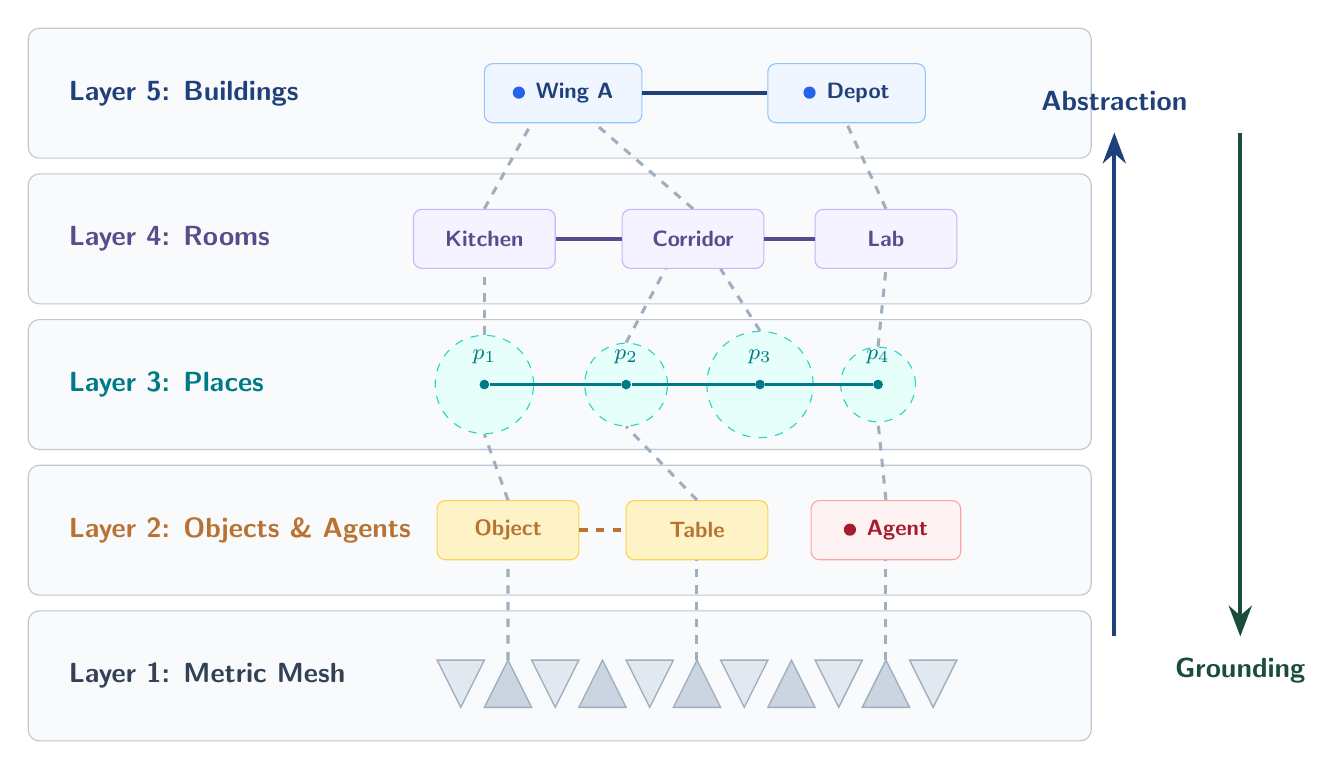
\begin{tikzpicture}[
    x=1cm, y=1cm,
    font=\sffamily\small,
    layer box/.style={draw=paleink!70, fill=cardbg, rounded corners=4pt, minimum width=13.5cm, minimum height=1.65cm, anchor=west},
    layer text/.style={font=\sffamily\bfseries, anchor=west},
    l5 node/.style={draw=l5nodeborder, fill=l5nodebg, rounded corners=3pt, minimum width=2.0cm, minimum height=0.75cm, text=l5text, font=\bfseries\footnotesize, align=center},
    l4 node/.style={draw=l4nodeborder, fill=l4nodebg, rounded corners=3pt, minimum width=1.8cm, minimum height=0.75cm, text=l4text, font=\bfseries\footnotesize, align=center},
    l2 obj/.style={draw=l2nodeborder, fill=l2nodebg, rounded corners=3pt, minimum width=1.8cm, minimum height=0.75cm, text=ethbronze, font=\bfseries\footnotesize, align=center},
    l2 agent/.style={draw=l2agentborder, fill=l2agentbg, rounded corners=3pt, minimum width=1.9cm, minimum height=0.75cm, text=harvardcrimson, font=\bfseries\footnotesize, align=center},
    l3 place/.style={circle, draw=l3sphereborder, dashed, fill=l3spherebg, inner sep=0pt, minimum size=1.1cm, align=center},
    l3 inner/.style={circle, fill=l3text, inner sep=0pt, minimum size=3.5pt},
    arrow/.style={-{Stealth[scale=1.2]}, line width=1.4pt},
    interlayer/.style={draw=paleink, line width=1.1pt, dashed},
    intraedge/.style={line width=1.3pt}
]

    % Coordinates for layers
    \foreach \y/\id in {0/1, 1.85/2, 3.7/3, 5.55/4, 7.4/5} {
        \node[layer box] (layer\id) at (0,\y) {};
    }

    % Layer 1: Metric Mesh
    \node[layer text, text=l1text] at ($(layer1.west) + (0.4,0)$) {Layer 1: Metric Mesh};
    \begin{scope}[shift={($(layer1.west) + (5.2,-0.4)$)}]
        \foreach \x in {0,1,...,10} {
            \pgfmathsetmacro{\xcoord}{\x*0.6}
            \pgfmathsetmacro{\nextx}{(\x+1)*0.6}
            \ifodd\x
                \filldraw[fill=l1trib, draw=paleink, line width=0.5pt] (\xcoord,0) -- (\xcoord+0.3,0.6) -- (\nextx,0) -- cycle;
            \else
                \filldraw[fill=l1tria, draw=paleink, line width=0.5pt] (\xcoord,0.6) -- (\xcoord+0.3,0) -- (\nextx,0.6) -- cycle;
            \fi
        }
        % Connection anchors on mesh aligned with Layer 2
        \coordinate (mesh1) at (0.9, 0.6);
        \coordinate (mesh2) at (3.3, 0.6);
        \coordinate (mesh3) at (5.7, 0.6);
    \end{scope}

    % Layer 2: Objects & Agents
    \node[layer text, text=l2text] at ($(layer2.west) + (0.4,0)$) {Layer 2: Objects \& Agents};
    \node[l2 obj] (l2obj1) at ($(layer2.west) + (6.1,0)$) {Object};
    \node[l2 obj] (l2obj2) at ($(layer2.west) + (8.5,0)$) {Table};
    \node[l2 agent] (l2agent) at ($(layer2.west) + (10.9,0)$) {\tikz{\fill[harvardcrimson] (0,0) circle(2.2pt);} \hspace{1pt}Agent};
    \draw[intraedge, ethbronze, dashed] (l2obj1) -- (l2obj2);

    % Layer 3: Places
    \node[layer text, text=l3text] at ($(layer3.west) + (0.4,0)$) {Layer 3: Places};
    
    \node[l3 place, minimum size=1.25cm] (p1) at ($(layer3.west) + (5.8,0)$) {};
    \node[l3 inner] (p1dot) at (p1.center) {};
    \node[text=l3text, font=\bfseries\footnotesize, above=2pt of p1dot] {$p_1$};

    \node[l3 place, minimum size=1.05cm] (p2) at ($(layer3.west) + (7.6,0)$) {};
    \node[l3 inner] (p2dot) at (p2.center) {};
    \node[text=l3text, font=\bfseries\footnotesize, above=2pt of p2dot] {$p_2$};

    \node[l3 place, minimum size=1.35cm] (p3) at ($(layer3.west) + (9.3,0)$) {};
    \node[l3 inner] (p3dot) at (p3.center) {};
    \node[text=l3text, font=\bfseries\footnotesize, above=2pt of p3dot] {$p_3$};

    \node[l3 place, minimum size=0.95cm] (p4) at ($(layer3.west) + (10.8,0)$) {};
    \node[l3 inner] (p4dot) at (p4.center) {};
    \node[text=l3text, font=\bfseries\footnotesize, above=2pt of p4dot] {$p_4$};

    \draw[intraedge, ethpetrol] (p1dot) -- (p2dot);
    \draw[intraedge, ethpetrol] (p2dot) -- (p3dot);
    \draw[intraedge, ethpetrol] (p3dot) -- (p4dot);
    
    % Layer 4: Rooms
    \node[layer text, text=l4text] at ($(layer4.west) + (0.4,0)$) {Layer 4: Rooms};
    \node[l4 node] (l4room1) at ($(layer4.west) + (5.8,0)$) {Kitchen};
    \node[l4 node] (l4room2) at ($(layer4.west) + (8.45,0)$) {Corridor};
    \node[l4 node] (l4room3) at ($(layer4.west) + (10.9,0)$) {Lab};
    \draw[intraedge, ethpurple] (l4room1) -- (l4room2);
    \draw[intraedge, ethpurple] (l4room2) -- (l4room3);

    % Layer 5: Buildings
    \node[layer text, text=l5text] at ($(layer5.west) + (0.4,0)$) {Layer 5: Buildings};
    \node[l5 node] (l5wing) at ($(layer5.west) + (6.8,0)$) {\tikz{\fill[l5nodedot] (0,0) circle(2.2pt);} \hspace{1pt}Wing A};
    \node[l5 node] (l5depot) at ($(layer5.west) + (10.4,0)$) {\tikz{\fill[l5nodedot] (0,0) circle(2.2pt);} \hspace{1pt}Depot};
    \draw[intraedge, ethdarkblue] (l5wing) -- (l5depot);
    
    % Vertical Inter-layer Edges (dashed)
    % Mesh to Objects
    \draw[interlayer] (mesh1) -- (l2obj1.south);
    \draw[interlayer] (mesh2) -- (l2obj2.south);
    \draw[interlayer] (mesh3) -- (l2agent.south);
    
    % Objects to Places
    \draw[interlayer] (l2obj1.north) -- (p1.south);
    \draw[interlayer] (l2obj2.north) -- (p2.south);
    \draw[interlayer] (l2agent.north) -- (p4.south);
    
    % Places to Rooms
    \draw[interlayer] (p1.north) -- (l4room1.south);
    \draw[interlayer] (p2.north) -- ($(l4room2.south) + (-0.35,0)$);
    \draw[interlayer] (p3.north) -- ($(l4room2.south) + (0.35,0)$);
    \draw[interlayer] (p4.north) -- (l4room3.south);

    % Rooms to Buildings
    \draw[interlayer] (l4room1.north) -- ($(l5wing.south) + (-0.4,0)$);
    \draw[interlayer] (l4room2.north) -- ($(l5wing.south) + (0.4,0)$);
    \draw[interlayer] (l4room3.north) -- (l5depot.south);

    % Right Panel: Flow
    \begin{scope}[shift={(14.6, 3.7)}]
        \draw[arrow, ethdarkblue] (-0.8, -3.2) -- (-0.8, 3.2);
        \node[font=\sffamily\bfseries, text=ethdarkblue, anchor=south] at (-0.8, 3.35) {Abstraction};
        
        \draw[arrow, emeraldpine] (0.8, 3.2) -- (0.8, -3.2);
        \node[font=\sffamily\bfseries, text=emeraldpine, anchor=north] at (0.8, -3.35) {Grounding};
    \end{scope}

\end{tikzpicture}
\end{document}
